\documentclass[10pt,a4paper]{article}
%\usepackage[ngerman]{babel}
\usepackage{color}
\usepackage{listings}
\usepackage{graphicx}
\usepackage{float}

\setlength{\parindent}{0pt}

\title{\textbf{Exercise 8 Group 14}}
\author{Jon Volkmar\\
		Heiko Baumann\\
		Peter Hirschfeld}
\date{}
\begin{document}

\maketitle

%\section{}

\begin{enumerate}
\item Please describe in your own words the difference between RDFS amd OWL, and 
then between OWL Lite, OWL DL, OWL Full and OWL 2. Create some simple 
examples to illustrate the difference.

\textbf{Answer:}
OWL is more expressive than RDFS: with OWL we can define relations between classes, constraints and cardinalities, equivalences of classes and properties, create properties of properties, use boolean combinations and other expressive constructs (e.g. disjointnes, inverse properties, property restrictions, enumerations). Also, special properties can be expressed, namely transitive, symmetric, functional, and inverse functional properties. However, some RDF markup is preserved in OWL, and instances of classes are declared in RDF.

OWL Lite is a simplified subset of OWL for tool developers, with some features from OWL, supporting class hierarchies and constraints.

OWL DL: DL stands for description logic. It is restricted compared to OWL Full in that classes cannot be simultaneously be properties and individuals, and properties cannot simultaneouly be individuals. This is called vocabulary partitioning. As well, the set of object properties and data type properties are disjoint in DL. DL also requires explicit typing. No transitive cardinality constraints can exist in OWL DL. Another difference is that there are some restrictions placed on the usage of anonymous classes.

OWL 2 has several new constructs, such as qualified cardinality restrictions, role chains, and expressive data predicates. It has some different syntaxes, and targets the XML technology toolchain with OWL/XML, which is a new non-RDF XML syntax. It has added features for supporting datatypes, metamodelling, annotation, and database style keys. Property chains are also introduced: for example saying that { ?x ex:uncle ?y } is equivalent to { ?x ex:parent ?z . ?z ex:brother ?y . }

\textbf{TODO Add examples}

\item Ontology modelling application scenario

\begin{enumerate}

\item Competency questions: Write down at least 20 competency questions which the intended application should be able to answer on the basis of the ontology.

\textbf{Answer:}

\begin{enumerate}

\item For a given course, who is the lecturer or tutor?
\item  How many students are enrolled in a given class?
\item Where and when is a lecture given?
\item What are the names of the courses a given student is enrolled in?
\item Which lectures occur on a given day of the week?
\item What are the names of the students enrolled for a given course?
\item How many times does a course occur per week?
\item How many instructors are there for a given course?
\item Who is allowed to loan a given faculty resource (e.g. room, projector, PC...)
\item For a given room, what dates is it booked for?
\item What is the maximum loan period for a given faculty resource?
\item Is a resource currently on loan?
\item What is the capacity of a given course?
\item Is a given course a lecture or a seminar?
\item What prior courses are required for a student to participate in a given courses?
\item Which courses is a student eligible to enroll for?
\item For a given student, which courses need to be completed before they can enroll in a certain course?
\item Which resources is a given person allowed to loan?
\item Is a particular resource loanable?
\item What are the names of all the students enrolled in a course which takes place on a Monday?
\end{enumerate}

\item Glossary: Extract key terms from the competency questions which frequently occur and are of importance for the given application domain. 

\textbf{Answer:}

\begin{itemize}
\item Course
\item Lecturer
\item Tutor
\item Student
\item Course Name
\item Course capacity
\item Loan period
\item Booked dates
\item Lecture 
\item Seminar
\item Required courses
\item Loanability
\end{itemize}

\item Mindmap: Create mindmaps to model the relationships between the key terms of your glossary in a light-weight way.

\textbf{Answer:}

Mindmap created with Freemind:

\begin{figure}[H]
  \caption{Mindmap of the "Faculty" ontology}
  \centering
    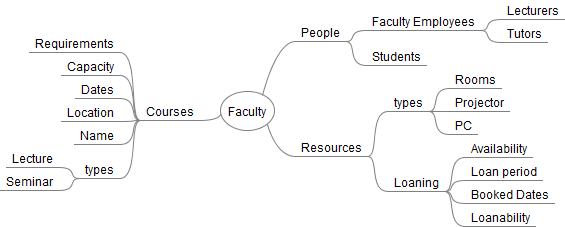
\includegraphics[scale=0.7]{Faculty_mindmap.png}
\end{figure}



\item Ontology engineering: Derive from the mindmaps an ontology containing some first classes. Use a ontology editor for this task, e.g., Protégé(http://protege.stanford.edu/). Add labels in English and German language to each concept of your ontology

\textbf{Answer:}

Ontology created with Protégé. Please see ex8.owl for the OWL/XML markup. The following diagram, generated by the OwlViz tool in Protégé, shows the classes of the ontology. It does not show the object and data properties which are used in restrictions fufilling our scenario requirements, to view these the owl file must be opened in Protege or simply in a text editor.

\begin{figure}[H]
  \caption{Classes in the OWL representation of the "Faculty" ontology}
  \centering
    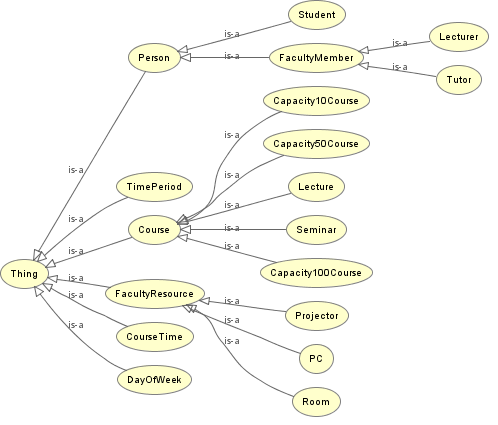
\includegraphics[scale=0.7]{owl_graph.png}
\end{figure}


\end{enumerate}

\end{enumerate}


\end{document}